\documentclass[12pt, oneside]{book}
\usepackage[paperwidth=216mm, paperheight=279mm,top=3cm, bottom=2.5cm, right=2.5cm, left=2.5cm]{geometry}
% Paquetes necesarios

\usepackage[utf8]{inputenc}
\usepackage[T1]{fontenc}
\usepackage[spanish, es-tabla]{babel} % Español

\usepackage{titlesec}
\usepackage{lipsum} 
\usepackage{setspace} 
\usepackage{hyperref}
\usepackage{graphicx}
\usepackage{float}
\usepackage{amssymb} 
\usepackage{amsmath}
\usepackage{etoolbox}
\usepackage{subcaption} 
\usepackage{array}
\usepackage{algorithm}
\usepackage{algpseudocode}
\usepackage{pgfplots}
\usepackage{adjustbox}
\usepackage{booktabs}
\usepackage{tabularx}
\usepackage[table,xcdraw]{xcolor}
\usepackage{enumitem}
\usepackage{csquotes}
\usepackage{longtable}
\usepackage{pdflscape}
\usepackage{graphicx}
\usepackage{float}
\usepackage{multicol}
\usepackage{multirow}


%para bibliografía en formato APA, requerido en biblioteca
\usepackage[style=apa,sortcites=true,sorting=nyt,backend=biber]{biblatex}
%\DeclareLanguageMapping{american}{american-apa} % para texto en inglés
\DeclareLanguageMapping{spanish}{spanish-apa}    % para texto en español

\addbibresource{bibliografia.bib}


%%%%% configuración de párrafos
\setlength{\parindent}{4em} %identación inicial
\raggedbottom %para evitar espacio grandes entre parrafos
%\setlength{\parskip}{0.7em} %separación entre párrafos

\renewcommand{\baselinestretch}{1.5} %separación entre lineas

\titleformat{name=\chapter}[display]{\filright\bfseries}{\Large\chaptername~\thechapter}{20pt}{\Huge}
\titlespacing*{name=\chapter}{0pt}{0pt}{20pt}


%\titleformat{\chapter}[display]
%  {\normalfont\Huge\bfseries}{}{0pt}{\fontsize{20}{22}\selectfont}
%\titlespacing*{\chapter}{0pt}{-20pt}{20pt}

\let\cleardoublepage\clearpage

\begin{document}

\begin{titlepage}
\begin{center}
\begin{figure}[h]
    \begin{center}
        
\includegraphics[height=3.75cm]{imagenes/EscudoEscuelaICI}
    \end{center}
\end{figure}

\vspace{4em} %6em

 {\huge\textsc{
Aplicación Móvil de Acompañamiento para Pacientes Oncológicos
}}\\

 \vspace{6em}
\textsc{Memoria para obtener el título de}\\

\textsc{INGENIERO CIVIL EN INFORMÁTICA}\\[4em]

\textsc{Autor}\\
\textsc{\Large Javier Ignacio Baeza Toro}\\
\textsc{\Large Angel Tómas Montecino Flores}\\[2em]

\textsc{Profesor guía}\\
\textsc{\large Dr. Miguel Esteban Romero Vásquez.}\\[2em]

\vspace*{\fill}

\textsc{Enero, 2026}\\
\textsc{Chillán-Chile}
\end{center}

\end{titlepage}


% Página en blanco después de la portada
\newpage
\thispagestyle{empty}
\mbox{}

\chapter*{Agradecimientos}

\subsection*{Felipe Esteban Toro Castro}




% Resumen
\chapter*{Resumen}

\chapter*{Abstract}
%This final degree project, developed within the framework of the Computer Civil Engineering program at the Universidad del Bío-Bío, is entitled “Fluxora: Business Management System to Optimize Distribution, Sales, and Inventory.” It arises as a response to the need to modernize the management processes of small and medium-sized production and distribution companies that still rely on manual records and traditional methods, making inventory control, production traceability, and delivery coordination difficult.

This undergraduate capstone project, entitled \textit{“xxx”}, was developed and submitted in partial fulfillment of the requirements for the undergraduate professional degree Ingeniería Civil en Informática at the University of Bío-Bío, a Chilean engineering program encompassing Computer Science, Software Engineering, and Information Systems. 

This project focuses on ...
% Índice
\tableofcontents
\listoftables
\listoffigures

% Capítulos
\chapter{Introducción}

%para citas en el texto se usa \textcite{Shotton1989}.  Por ejemplo:
%            cómo señala \textcite{Shotton1989}... 
%   produce: como señala Shotton (1989)
% para citas con paréntesi se usa \parencite{Shotton1989}, que son las ejemplificadas más abajo.
%las referencias bibliográficas se agregan en el archivo bibliografia.bib en formato bibtex.


\chapter{Definición de la empresa}

\section{Descripción de la empresa}

A continuación se presentan los antecedentes institucionales y la identificación formal del establecimiento asistencial de referencia \parencite{hchm2024web}:

\begin{itemize}
    \item \textbf{Nombre:} Hospital Clínico Herminda Martín (HCHM)
    \item \textbf{RUT:} 61.607.001-0 (Establecimiento de salud pública autogestionado en red)
    \item \textbf{Dirección principal (Chillán):} Av. Francisco Ramírez N° 10, Chillán, Región de Ñuble
    \item \textbf{Dependencia institucional:} Servicio de Salud Ñuble, Ministerio de Salud de Chile (MINSAL) \parencite{minsal2022plancancer}
    \item \textbf{Entorno clínico de referencia:} Unidad de Oncología / Centro Ambulatorio de Especialidades (CAE) -- Unidad de Quimioterapia Ambulatoria
    \item \textbf{Dirección del establecimiento:} Dra. Luz María Morán Ibáñez
    \item \textbf{Teléfonos de contacto:} Central telefónica: +56 42 258 6400 | OIRS: +56 42 258 6765
\end{itemize}

\section*{Historia de la empresa}
El Hospital Clínico Herminda Martín de Chillán constituye el principal centro asistencial de alta complejidad y de referencia técnica para la Región de Ñuble. Su origen se remonta al período comprendido entre 1941 y 1945, originado tras el terremoto de 1939 que destruyó el antiguo Hospital San Juan de Dios. La edificación del recinto hospitalario fue posible gracias a la donación testamentaria de doña Herminda Martín Mieres, benefactora que legó los recursos financieros destinados a dotar a la provincia de un moderno establecimiento de salud \parencite{hchm2024web}.

A lo largo de su historia asistencial, el recinto expandió sistemáticamente sus dependencias y cartera de servicios. En la década de 1970 se habilitó el Consultorio Adosado de Especialidades (CAE) y, en la década de 1990, se integraron la Unidad de Paciente Crítico (UPC) y la actual Unidad de Emergencia. Posterior a los daños estructurales provocados por el terremoto de febrero de 2010, el hospital completó un plan integral de normalización y reconstrucción que restituyó su operatividad bajo estándares sismorresistentes \parencite{hchm2024web}.

En el ámbito oncológico, el HCHM consolidó la Unidad de Quimioterapia Ambulatoria dentro del Servicio de Oncología, estableciéndose como el nodo operativo central para la infusión y control de tratamientos sistémicos antineoplásicos e inmunoterapias dirigidos a la población de las 21 comunas que integran la Región de Ñuble \parencite{minsal2022plancancer}.

\section*{Misión}
«Ofrecer una atención integral y de calidad, que contribuye a la recuperación de la salud de las personas, trabajando en equipo, comprometidos e integrados a la red asistencial» \parencite{hchm2024web}.

\section*{Visión}
«Ser un hospital clínico, líder en innovación, para satisfacer las necesidades de salud y elevar la calidad de vida de la comunidad, en forma participativa e inclusiva; con el compromiso de sus trabajadores» \parencite{hchm2024web}.

\section*{Descripción del área de estudio}
El presente proyecto se focalizó exclusivamente en la \textbf{Unidad de Quimioterapia Ambulatoria}, unidad funcional adscrita al Servicio de Oncología y al Centro Ambulatorio de Especialidades (CAE) del Hospital Clínico Herminda Martín. Dicha dependencia concentra los procedimientos de administración parenteral de esquemas citostáticos, terapias biológicas dirigidas y el seguimiento de toxicidades farmacológicas en pacientes oncológicos adultos.

La dinámica operativa de esta unidad presenta una modalidad ambulatoria: el paciente concurre a su sesión de infusión citotóxica en el recinto hospitalario y posteriormente retorna a su domicilio para cursar el período inter-ciclo (comprendido habitualmente entre 14 y 28 días). Durante este lapso domiciliario, el monitoreo y reporte de complicaciones recaen de manera autónoma en el propio paciente o en su cuidador informal.

Por consideraciones asistenciales y de alcance técnico, el área de radioterapia fue excluida del proyecto por dos razones determinantes:
\begin{enumerate}
    \item \textbf{Carencia de infraestructura local y derivación a la macrored:} El Hospital Clínico Herminda Martín no cuenta con equipamiento ni búnker de radioterapia en sus instalaciones de Chillán. Como se constató en las entrevistas al equipo clínico, los pacientes que requieren radioterapia o exámenes de alta complejidad deben ser derivados a prestadores de compra o a centros de la macrored asistencial en la ciudad de Concepción. Por el contrario, la quimioterapia se prepara, administra y controla íntegramente en las dependencias del HCHM.
    \item \textbf{Diferencia en el patrón de toxicidad:} Las complicaciones de la radioterapia corresponden a cuadros loco-regionales con dinámicas asistenciales distintas, mientras que la quimioterapia sistémica induce toxicidades agudas, fluctuaciones hematológicas severas (nadir) y riesgo de descompensación inter-ciclo diario que demandaron un motor de seguimiento continuo y triaje perimetral \parencite{minsal2022plancancer}.
\end{enumerate}

\section{Descripción del problema}
Durante el levantamiento de requerimientos y la observación en terreno en la Unidad de Quimioterapia del HCHM, se evidenció una brecha operacional crítica entre el egreso de la sala de infusión y el reingreso al siguiente ciclo de tratamiento. Como manifestó el personal clínico durante las sesiones de levantamiento técnico: \textit{«nosotros trabajamos muy estrictamente porque los sistemas no nos ayudan»} \parencite{entrevistaHCHM2026}.

El análisis del flujo asistencial reveló factores determinantes que fundamentaron la necesidad de desarrollar una solución tecnológica desacoplada y centrada en el paciente:

\begin{enumerate}
    \item \textbf{Brecha de alfabetización en salud y sobrecarga cognitiva:} En los talleres de inducción a la quimioterapia se identificó que los pacientes enfrentan una barrera importante en la comprensión de su patología y del tratamiento médico, señalando el equipo de salud:
    \begin{quote}
        \textit{«Cuando nosotros vamos al taller de ingreso, los pacientes no saben ni qué es el cáncer... No saben que son células, no saben que proliferan, no saben nada de eso... De tratamiento tampoco saben, no saben qué [es] adyuvante, les dicen: usted va a hacer una quimioterapia neoadyuvante, claro, le hablan en chino [...], pero no le dicen que es una quimio que es antes de la cirugía y con qué propósito está esa quimioterapia»} \parencite{entrevistaHCHM2026}.
    \end{quote}
    Este déficit educativo basal, sumado al impacto del deterioro cognitivo transitorio y fatiga oncológica inducida por fármacos, exigió descartar interfaces complejas en favor de un diseño accesible guiado por la heurística de tres pasos de interacción:
    \begin{quote}
        \textit{«Tenía los 3 clic y eso es lo que tiene que visualizar, los 3 clic son 3 clic que hace para llegar a lo que quiere buscar [...] la gracia es que sea lo más fácil posible, lo más amigable posible, porque [...] si ya no saben de parte de lo que es el cáncer, quizás lo más probable es que tampoco manejen tanto la tecnología. Por eso hay que hacerlo simple nomás»} \parencite{entrevistaHCHM2026}.
    \end{quote}
    Este principio de reducción de costo cognitivo responde a las directrices de usabilidad y accesibilidad priorizadas directamente por el equipo asistencial durante el levantamiento técnico en terreno \parencite{entrevistaHCHM2026}.

    \item \textbf{Dispersión geográfica y brecha de conectividad digital:} De acuerdo con los antecedentes del Censo Oficial y el Plan Nacional de Cáncer, la Región de Ñuble presenta una de las tasas de ruralidad más altas del país junto con los menores niveles de ingreso autónomo \parencite{ine2024censo, minsal2022plancancer}. Gran parte de los pacientes atendidos provienen de sectores rurales con cobertura móvil deficiente o nula. Ante complicaciones críticas como la neutropenia febril (temperatura axilar $\ge 38,0^\circ\text{C}$) en los días de nadir hematológico (días 7 a 14 post-infusión), depender de conectividad continua a servidores en la nube representó un riesgo vital severo \parencite{minsal2022plancancer}.

    \item \textbf{Restricciones clínicas en modelos conversacionales y resguardo de datos:} El equipo clínico enfatizó que la interacción digital debe resguardar estrictamente la privacidad de los datos sensibles y restringir el uso de modelos generativos abiertos que puedan desorientar al usuario:
    \begin{quote}
        \textit{«Primero súper resguardando los datos y lo otro que tampoco promueva, ponte tú, porque acá qué puede pasar que el paciente [...] tenga sintomatología depresiva por la condición en sí. Entonces puede decir me siento mal, no sé qué quiero hacer tal cosa y si la cuestión le afirma, le refuerza más la situación, entonces eso tenemos que evitarlo completamente [...] Y tú crees que los modelos en el fondo siempre como que te dan la razón. Entonces eso igual es un riesgo»} \parencite{entrevistaHCHM2026}.
    \end{quote}
    Esto fundamentó la implementación de un motor de triaje determinista local (\textit{edge computing}) basado en árboles de decisión clínicos cerrados y cuestionarios estructurados condicionales \parencite{entrevistaHCHM2026}, independiente de servicios de procesamiento de lenguaje en la nube para la evaluación de urgencias.

    \item \textbf{Sobrecarga de datos no estructurados y latencia en la toma de decisión médica:} Durante el levantamiento de requerimientos en terreno, se constató que el personal asistencial carecía de mecanismos automatizados para sintetizar los eventos clínicos acumulados durante el período inter-ciclo \parencite{entrevistaHCHM2026}. La revisión manual de registros extensos con predominio de mediciones fisiológicas dentro de rangos normales representaba una sobrecarga informativa inoperativa para el tiempo acotado de la consulta médica. Por ello, el equipo de salud planteó la necesidad crítica de contar con una herramienta de reportabilidad clínica orientada a jerarquizar y filtrar de forma inmediata exclusivamente las variables alteradas y signos de alerta, suprimiendo la dependencia de relatos orales retrospectivos e imprecisos durante la reevaluación del paciente \parencite{entrevistaHCHM2026}.
\end{enumerate}

\newpage
\begin{landscape}
\thispagestyle{empty}

\vspace*{\fill}
\centering
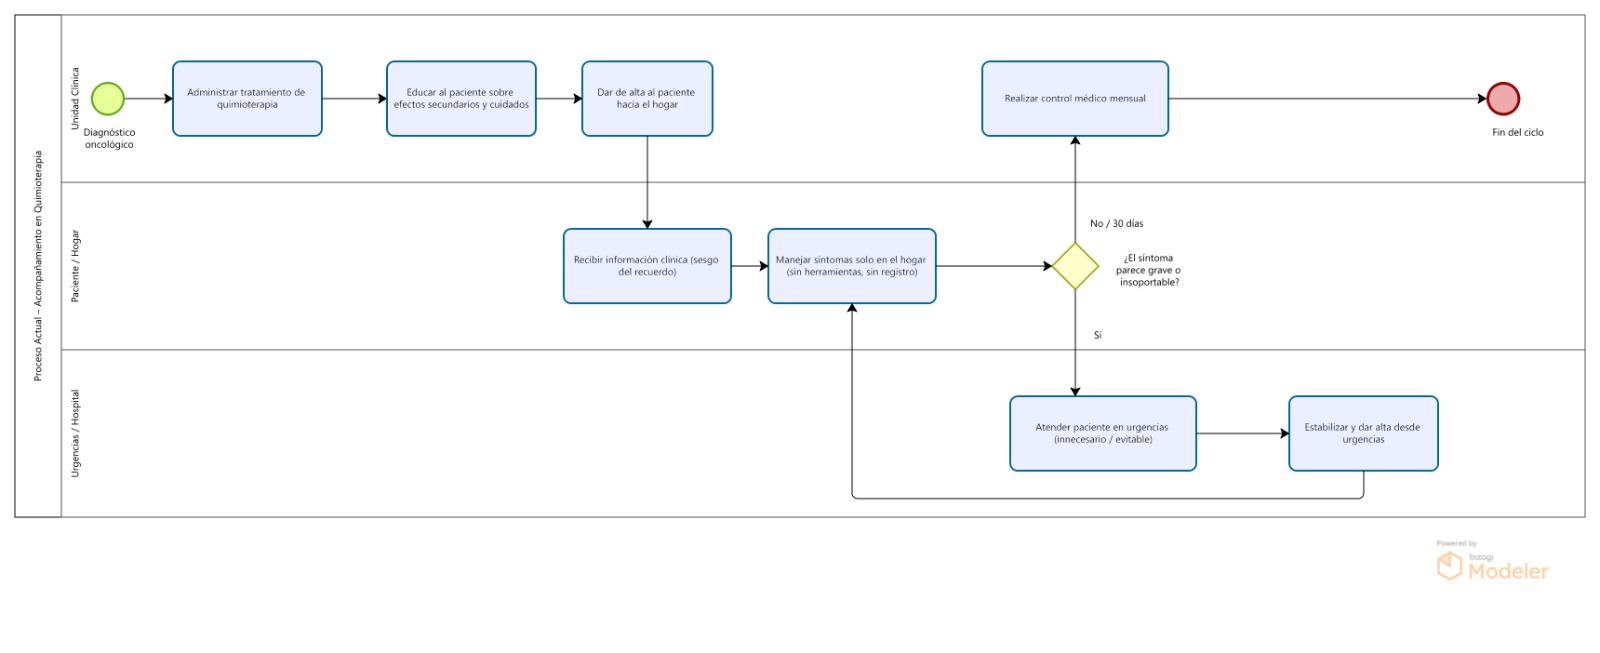
\includegraphics[
    width=1.1\paperwidth,
    height=1.1\paperheight,
    keepaspectratio
]{imagenes/bpmn_oncologia.png}

\captionof{figure}{Proceso de negocio “Acompañamiento en Oncología”}
\label{fig:BPMN Acompanamiento}
\vspace*{\fill}

\end{landscape}

\noindent
\textbf{BPMN 1 – Proceso actual de acompañamiento Oncológico (Figura \ref{fig:BPMN Acompanamiento})}

\noindent
El modelado del proceso de negocio evidenció el flujo operativo mediante el cual se ejecutaba el seguimiento de los pacientes en la Unidad de Quimioterapia del HCHM:

\noindent
El proceso se iniciaba al concluir la infusión citostática en la sala de quimioterapia. El personal de enfermería entregaba indicaciones verbales y folletos impresos con recomendaciones generales de autocuidado. A partir de ese momento, el paciente regresaba a su domicilio, asumiendo de manera autónoma la vigilancia y el registro de sus síntomas durante el período inter-ciclo.

\noindent
Ante la manifestación de toxicidades severas o alzas térmicas, el flujo dependía exclusivamente de la iniciativa del paciente o de su red de apoyo para trasladarse espontáneamente al Servicio de Urgencia del hospital o comunicarse telefónicamente. Al ingresar a la urgencia, el paciente se sometía al triage general sin disponer de un historial estructurado ni registro evolutivo de los parámetros fisiológicos previos, lo que demoraba la categorización médica y la identificación oportuna del nadir hematológico \parencite{minsal2022plancancer, entrevistaHCHM2026}.

\vspace{0.7cm}

\subsection*{Problemas detectados}
A partir de la triangulación entre la observación en terreno, las entrevistas semiestructuradas con el personal clínico del HCHM \parencite{entrevistaHCHM2026} y la revisión del Plan Nacional de Cáncer \parencite{minsal2022plancancer}, se consolidaron los siguientes problemas estructurales del área de estudio:

\begin{enumerate}
    \item \textbf{Latencia crítica en la identificación de toxicidades agudas:} La ausencia de un registro diario sistemático generó que complicaciones graves (neutropenia febril, deshidratación severa) fueran detectadas tardíamente, aumentando los ingresos de urgencia en estados clínicos deteriorados \parencite{minsal2022plancancer, entrevistaHCHM2026}.
    \item \textbf{Inoperatividad de soluciones dependientes de conectividad en red rural:} Debido a la alta dispersión y ruralidad en la Región de Ñuble, los sistemas basados exclusivamente en servicios en la nube quedaban inoperativos en zonas sin cobertura celular, impidiendo la emisión oportuna de alertas de riesgo en el hogar del paciente \parencite{ine2024censo, minsal2022plancancer}.
    \item \textbf{Ausencia de un motor de triaje determinista perimetral (\textit{edge}):} El entorno clínico no contaba con una solución móvil capaz de procesar signos vitales y síntomas de forma local e independiente de la red, imposibilitando la entrega de clasificaciones de gravedad inmediatas ante emergencias oncológicas.
    \item \textbf{Barrera de usabilidad en pacientes con fatiga y sobrecarga cognitiva:} Las herramientas digitales convencionales resultaban inadecuadas para pacientes sometidos a quimioterapia que presentaban cuadros de fatiga extrema o deterioro cognitivo leve transitorio, exigiendo una arquitectura de información simplificada y restringida a un máximo de tres pasos de interacción por flujo \parencite{entrevistaHCHM2026}.
    \item \textbf{Inexistencia de reportabilidad clínica estructurada:} La sobrecarga asistencial del equipo médico impedía la revisión manual de historiales extensos, haciendo necesaria una herramienta que consolidara y priorizara exclusivamente las variables fuera de rango clínico para optimizar la toma de decisiones en los controles de ciclo \parencite{entrevistaHCHM2026}.
\end{enumerate}
\chapter{Definición del proyecto}

\section{Objetivos del proyecto}

\subsection*{Objetivo General}

Desarrollar el módulo móvil de una plataforma integrada de acompañamiento oncológico domiciliario, mediante una aplicación Android con arquitectura offline-first y motor de triaje edge local, que permitió a pacientes en tratamiento de quimioterapia registrar síntomas y signos vitales sin depender de conectividad, recibir alertas de urgencia evaluadas localmente en el dispositivo, y acceder al contenido educativo y al asistente conversacional del sistema.

\subsection*{Objetivos Específicos}
\begin{enumerate}
    \item \textbf{Interfaz y Accesibilidad:} Se diseñó e implementó una aplicación móvil Android en React Native con Expo, accesible para pacientes con fatiga cognitiva, con módulos de registro de síntomas y signos vitales, biblioteca educativa y acceso al asistente conversacional, garantizando un máximo de 3 interacciones para alcanzar cualquier función principal.
    \item \textbf{Motor de Triaje Edge:} Se construyó un motor de triaje edge local que evaluó en tiempo real los signos vitales registrados en el dispositivo, emitiendo alertas de urgencia sin requerir conexión a internet, y derivando automáticamente al paciente a atención médica ante la detección de valores críticos o palabras clave de riesgo.
    \item \textbf{Arquitectura Offline-First:} Se implementó una arquitectura offline-first mediante SQLite local (expo-sqlite) y sincronización bidireccional diferida con PowerSync, garantizando que los registros de síntomas persistieran íntegramente en el dispositivo durante períodos sin conectividad y se sincronizaran automáticamente sin duplicación con la base central de la plataforma al recuperar señal.
    \item \textbf{Backend Pasarela:} Se desarrolló un backend de pasarela (gateway) en Node.js + Express que gestionó notificaciones push, sesiones de dispositivo y consumo autenticado de la API clínica central mediante el token JWT emitido por el módulo de inteligencia clínica, sin replicar lógica de autenticación de usuarios.
    \item \textbf{Motor Nativo de Reportes:} Se implementó un motor nativo de generación de reportes que exportó el historial de síntomas y signos vitales en formato PDF y Excel directamente desde el dispositivo, incluyendo el código único de vinculación del paciente para su presentación al equipo médico en controles programados.
    \item \textbf{Evaluación Técnica y Robustez:} Se evaluó la robustez del motor de triaje edge y la integridad de la sincronización offline-first ante escenarios de desconexión prolongada y valores clínicos límite, midiendo la tasa de falsos negativos/positivos en alertas críticas y la tasa de conflictos resueltos correctamente durante la sincronización diferida.
\end{enumerate}

\section{Ambiente de Ingeniería de Software}

\subsection*{Metodología de trabajo}

Se utilizó Scrum como marco de trabajo ágil, dada la necesidad de un desarrollo iterativo e incremental. Los requerimientos se priorizaron según su impacto en la seguridad clínica del paciente (Alta, Media, Baja), permitiendo entregas funcionales constantes. La planificación de los sprints y el diseño de API se coordinó directamente con el equipo responsable del módulo de inteligencia clínica y plataforma web.

\subsection*{Arquitectura del sistema}

\subsection*{Justificación de la arquitectura seleccionada}

La arquitectura offline-first se justificó por la necesidad de garantizar disponibilidad del registro de síntomas y de la evaluación de triaje en zonas rurales de la región de Ñuble con conectividad intermitente. La separación entre el gateway del módulo móvil y la API clínica central permitió que el equipo de desarrollo del Módulo Móvil no dependiera de replicar lógica de autenticación ni el motor de inteligencia artificial RAG, responsabilidad del módulo de plataforma web (Jiménez \& Muñoz, 2026).

\subsection*{Evaluación de Impacto y Compromisos}


\section{Tecnologías Utilizadas}

\subsection*{Aplicación móvil:}
\begin{itemize}
    \item \textbf{React Native + Expo:} Se utilizó como framework principal del cliente móvil, permitiendo compilar una aplicación nativa para Android a partir de una base de código tipada en TypeScript. Expo proporcionó acceso simplificado a funcionalidades del dispositivo como sistema de archivos, notificaciones locales y SQLite embebido.
    \item \textbf{TypeScript:} Se empleó en todo el stack (móvil, gateway) para añadir tipado estático, mejorando la detección de errores y la mantenibilidad del código.
    \item \textbf{Expo Router:} Se utilizó para gestionar la navegación interna entre pantallas de la aplicación.
    \item \textbf{expo-sqlite:} Se integró como motor relacional embebido para garantizar la disponibilidad total del registro de síntomas sin conexión a internet (RNF-04).
    \item \textbf{expo-file-system / expo-notifications:} Se utilizaron para la gestión de archivos de reportes generados en cliente y para las notificaciones push y recordatorios locales, respectivamente.
\end{itemize}

\subsection*{Motor de triaje edge local:}
\begin{itemize}
    \item Se implementó de forma nativa en el dispositivo en TypeScript, procesando de forma síncrona y local los datos ingresados en expo-sqlite, comparándolos contra la matriz de umbrales fisiológicos validados por el equipo de enfermería, sin realizar peticiones HTTP ni depender de conectividad.
    \item Cada resultado emitido se registró localmente en la tabla \texttt{EVALUACION\_TRIAJE} (fecha, nivel de alerta, parámetro gatillante y derivación), permitiendo la auditoría histórica de eventos críticos.
\end{itemize}

\subsection*{Backend de pasarela (gateway):}
\begin{itemize}
    \item \textbf{Node.js + Express (TypeScript):} Se utilizó para implementar el servidor intermedio entre la aplicación móvil, los servicios de notificaciones y la API clínica central.
    \item \textbf{jsonwebtoken:} Se empleó para validar la firma y vigencia del token JWT emitido por el backend central en cada petición, retornando un código HTTP 401 ante un token expirado o inválido.
    \item \textbf{Prisma ORM + PostgreSQL:} Se utilizó una instancia liviana de PostgreSQL gestionada con Prisma ORM para la gestión de sesiones de dispositivo (\texttt{SESION\_DISPOSITIVO}) y el registro de tokens push, aislando estos datos operativos de la base de datos clínica central.
    \item \textbf{Axios, CORS, Helmet:} Se utilizaron para la comunicación saliente hacia la API central y para reforzar la seguridad HTTP del servicio.
\end{itemize}

\subsection*{Base de datos y sincronización:}
\begin{itemize}
    \item \textbf{PowerSync:} Se utilizó para ejecutar la sincronización bidireccional diferida entre la base de datos SQLite local del dispositivo móvil y la base de datos PostgreSQL central de la plataforma integrada, gestionando una arquitectura offline-first transparente sin intervención manual del paciente.
\end{itemize}

\subsection*{Gestión de estado, validación y exportación nativa:}
\begin{itemize}
    \item \textbf{Zustand:} Se utilizó para la gestión del estado global, garantizando reactividad liviana en el cliente móvil.
    \item \textbf{Zod:} Se empleó para centralizar la validación de la estructura de los datos de entrada y salida.
    \item \textbf{jsPDF:} Se utilizó para la exportación del historial de síntomas en formato PDF directamente en el cliente.
    \item \textbf{SheetJS (XLSX):} Se empleó para la generación de hojas de cálculo, incorporando el código único de vinculación en el encabezado.
\end{itemize}

\subsection*{Pruebas:}
\begin{itemize}
    \item \textbf{Vitest (TypeScript):} Se utilizó como framework de pruebas unitarias e integración para el motor de triaje edge, los formateadores de reportes y los middlewares de validación JWT en el gateway.
\end{itemize}

\subsection*{Definiciones, Siglas y Abreviaciones:}
\begin{itemize}
    \item \textbf{Offline-first:} Enfoque de diseño en el que la aplicación funciona completamente desde una base de datos local en el dispositivo, sincronizando con el servidor en segundo plano al recuperar conectividad.
    \item \textbf{Edge computing:} Paradigma que ejecuta la lógica de cómputo directamente en el dispositivo del usuario final, en lugar de depender de un servidor remoto.
    \item \textbf{JWT:} (JSON Web Token). Estándar abierto para la transmisión segura de información entre partes en forma de un objeto compacto y firmado digitalmente.
    \item \textbf{API REST:} Estilo de arquitectura para diseñar servicios web mediante el protocolo HTTP, utilizado para la comunicación entre el gateway del módulo móvil y la API clínica central.
    \item \textbf{RAG:} (Retrieval-Augmented Generation). Técnica de inteligencia artificial que combina un modelo de lenguaje generativo con un sistema de recuperación de información sobre un corpus controlado.
\end{itemize}
\chapter{Especificación de requerimientos}

\section{Alcances y limitaciones}

\subsection{Alcances}
El presente proyecto abarca el diseño, desarrollo, verificación y empaquetado del módulo móvil de la plataforma \textbf{QuimioCare}, enfocado exclusivamente en el acompañamiento ambulatorio de pacientes adultos en tratamiento de \textbf{quimioterapia}. El alcance específico comprende:

\begin{enumerate}
    \item \textbf{Aplicación móvil Android nativa:} Desarrollo en React Native con Expo SDK 57 y TypeScript, generando una \textit{Development Build} y compilación \textit{Release} demostrativa independiente con identificador de paquete \texttt{cl.ubiobio.quimiocare}.
    \item \textbf{Arquitectura Offline-First estricta:} Persistencia relacional en el dispositivo mediante SQLite (\texttt{expo-sqlite}) con migraciones versionadas (\texttt{001} a \texttt{008}), transacciones ACID y modo WAL, garantizando la captura y consulta ininterrumpida de signos vitales, síntomas libres, cuestionarios médicos asignados y contexto clínico sin requerir conexión a internet.
    \item \textbf{Aislamiento de perfiles de prueba:} Soporte determinista para dos pacientes sintéticos de demostración (Paciente A y Paciente B), garantizando que las bases de datos, copias de archivos locales y recordatorios mantengan estricta separación de pertenencia.
    \item \textbf{Gestión de copias educativas locales:} Descarga, almacenamiento atómico y lectura sin conexión de guías e infografías educativas en almacenamiento privado (\texttt{expo-file-system}), con reconciliación bidireccional de estados y visualización en línea de contenidos audiovisuales alojados en YouTube.
    \item \textbf{Motor nativo de reportes clínicos:} Consolidación histórica de mediciones y síntomas en ventanas de 7, 30 y 90 días, con generación y exportación local de documentos PDF (mediante \texttt{expo-print} con plantillas sanitizadas) y planillas de cálculo Excel (\texttt{.xlsx} con SheetJS), incorporando el código único de vinculación del paciente para su presentación en controles médicos.
    \item \textbf{Coordinador local de recordatorios:} Planificación nativa de notificaciones de medicamentos y controles mediante \texttt{expo-notifications} en una ventana móvil de 14 días (hasta 128 trabajos lógicos), operativa de forma autónoma sin la aplicación en ejecución.
    \item \textbf{Frontera de integración diferida:} Registro atómico de cada evento clínico en una cola local de envío (\texttt{cola\_envio}) con UUID idempotente, preparada para su futura transmisión REST hacia la pasarela o el simulador central.
\end{enumerate}

\subsection{Limitaciones}

\subsubsection{Limitaciones de Hardware y Software}
\begin{enumerate}
    \item \textbf{Plataforma de destino:} El desarrollo y la validación nativa se acotan a dispositivos móviles con sistema operativo Android versión 12 (API 31) o superior. El ecosistema iOS queda fuera del alcance de este ciclo.
    \item \textbf{Dependencia de conectividad para video:} Los recursos audiovisuales alojados en YouTube requieren conexión a internet para su reproducción externa; la aplicación no descarga ni almacena localmente archivos de video para respetar derechos de autor y políticas de almacenamiento.
    \item \textbf{Procesamiento de lenguaje natural y modelos generativos:} La aplicación no ejecuta modelos de lenguaje (LLM) ni motores RAG en el hardware del dispositivo. El asistente opera en el cliente mediante un controlador con estados deterministas y disclaimers visibles; la generación avanzada de respuestas queda delegada al servicio central.
\end{enumerate}

\subsubsection{Limitaciones Operativas y Clínicas}
\begin{enumerate}
    \item \textbf{Exclusión de radioterapia:} El módulo excluye flujos, tablas y contenidos de radioterapia, debido a que el Hospital Clínico Herminda Martín no dispone de equipamiento de radioterapia en Chillán (derivando pacientes a Concepción) y a que su dinámica asistencial difiere radicalmente de las toxicidades agudas de la quimioterapia sistémica.
    \item \textbf{Principio de no intervención clínica autónoma:} La aplicación es una herramienta de registro, educación y acompañamiento; no emite diagnósticos, no sugiere cambios de dosis ni reemplaza la evaluación médica presencial de urgencias.
    \item \textbf{Autoridad en la definición de cuestionarios:} Los formularios clínicos (tales como QLQ-C30 y ESAS) son diseñados y asignados exclusivamente por el equipo de salud en el backend central; el paciente responde las preguntas vigentes pero no edita plantillas clínicas.
\end{enumerate}

\section{Planificación de reuniones con el cliente y levantamiento}
El levantamiento de requerimientos se fundamentó en sesiones técnicas y entrevistas cualitativas con el personal clínico de la Unidad de Quimioterapia Ambulatoria del Hospital Clínico Herminda Martín (HCHM) de Chillán, junto con la revisión del Plan Nacional de Cáncer y la coordinación con el equipo del módulo web y de inteligencia clínica. Dichas interacciones permitieron identificar las siguientes directrices esenciales:
\begin{itemize}
    \item Priorizar la simpleza de uso y minimizar la sobrecarga cognitiva mediante la heurística de \textit{máximo 3 interacciones} para alcanzar cualquier función principal.
    \item Asegurar funcionamiento completo sin señal móvil para dar cobertura a la alta ruralidad de la Región de Ñuble.
    \item Incorporar de forma obligatoria avisos de responsabilidad clínica y la exportación de reportes físicos para el control médico presencial.
\end{itemize}

\section{Requerimientos funcionales}

A continuación se presentan los requerimientos funcionales del módulo móvil agrupados por subsistema:

% --- TABLA REGISTRO CLÍNICO Y VITALES ---
\begin{table}[H]
\centering
\renewcommand{\arraystretch}{1.3}
\setlength{\tabcolsep}{6pt}
\begin{tabularx}{\textwidth}{|c|p{3.5cm}|X|c|}
\hline
\textbf{ID} & \textbf{Nombre} & \textbf{Descripción} & \textbf{Prioridad} \\ \hline
RF\_01 & Registrar signos vitales & El sistema debe permitir registrar mediciones de presión arterial (sistólica/diastólica), pulso cardíaco, temperatura axilar y saturación de oxígeno, admitiendo entradas parciales y guardándolas de forma atómica en SQLite. & Alta \\ \hline
RF\_02 & Registrar síntomas diarios & El sistema debe permitir redactar una descripción libre de síntomas y malestares de hasta 2.000 caracteres, registrando la fecha y hora exacta sin requerir conexión a internet. & Alta \\ \hline
RF\_03 & Responder cuestionarios médicos & El sistema debe presentar formularios y encuestas médicas asignadas (ej. QLQ-C30, ESAS), permitiendo guardar borradores locales editables y confirmar entregas inmutables. & Alta \\ \hline
RF\_04 & Consultar historial clínico & El sistema debe mostrar el historial cronológico de mediciones y síntomas con filtros temporales de 7, 30 y 90 días y cálculo de estadísticas descriptivas. & Alta \\ \hline
\end{tabularx}
\caption{Requerimientos funcionales – Registro clínico y seguimiento}
\label{tab:rf_clinico}
\end{table}

% --- TABLA EDUCACIÓN Y ASISTENCIA ---
\begin{table}[H]
\centering
\renewcommand{\arraystretch}{1.3}
\setlength{\tabcolsep}{6pt}
\begin{tabularx}{\textwidth}{|c|p{3.5cm}|X|c|}
\hline
\textbf{ID} & \textbf{Nombre} & \textbf{Descripción} & \textbf{Prioridad} \\ \hline
RF\_05 & Consultar catálogo educativo & El sistema debe organizar recursos educativos en categorías temáticas sobre quimioterapia, cuidados y nutrición. & Alta \\ \hline
RF\_06 & Descarga y lectura de copias offline & El sistema debe permitir guardar copias locales de infografías y guías en almacenamiento persistente para lectura sin red, gestionando su eliminación y espacio utilizado. & Alta \\ \hline
RF\_07 & Visualizar videos de YouTube & El sistema debe permitir abrir enlaces directos a videos informativos en la aplicación de YouTube o navegador externo cuando exista conexión a internet. & Media \\ \hline
RF\_08 & Interacción con asistente conversacional & El sistema debe ofrecer una interfaz de chat asistivo con estados deterministas, cancelación de solicitudes y aviso permanente de responsabilidad médica. & Media \\ \hline
\end{tabularx}
\caption{Requerimientos funcionales – Educación y Asistencia}
\label{tab:rf_educacion}
\end{table}

% --- TABLA REPORTES Y RECORDATORIOS ---
\begin{table}[H]
\centering
\renewcommand{\arraystretch}{1.3}
\setlength{\tabcolsep}{6pt}
\begin{tabularx}{\textwidth}{|c|p{3.5cm}|X|c|}
\hline
\textbf{ID} & \textbf{Nombre} & \textbf{Descripción} & \textbf{Prioridad} \\ \hline
RF\_09 & Generar reporte PDF local & El sistema debe construir un documento PDF imprimible con las mediciones y síntomas del período seleccionado, incluyendo identificación y código de vinculación. & Alta \\ \hline
RF\_10 & Exportar reporte a Excel & El sistema debe generar una planilla de cálculo (.xlsx) estructurada con los registros clínicos del paciente para su procesamiento o auditoría médica. & Alta \\ \hline
RF\_11 & Compartir reportes externamente & El sistema debe invocar la hoja de compartición nativa de Android para enviar o guardar los archivos PDF y Excel generados. & Alta \\ \hline
RF\_12 & Gestionar recordatorios locales & El sistema debe permitir configurar horarios de medicación y controles, planificando notificaciones nativas en una ventana móvil de 14 días. & Alta \\ \hline
RF\_13 & Bandeja de avisos del paciente & El sistema debe proveer una vista centralizada de los avisos programados y pasados con acceso directo a la acción asociada. & Media \\ \hline
\end{tabularx}
\caption{Requerimientos funcionales – Reportes y Recordatorios}
\label{tab:rf_reportes_recordatorios}
\end{table}

% --- TABLA IDENTIDAD Y CONFIGURACIÓN ---
\begin{table}[H]
\centering
\renewcommand{\arraystretch}{1.3}
\setlength{\tabcolsep}{6pt}
\begin{tabularx}{\textwidth}{|c|p{3.5cm}|X|c|}
\hline
\textbf{ID} & \textbf{Nombre} & \textbf{Descripción} & \textbf{Prioridad} \\ \hline
RF\_14 & Aislamiento de paciente (A/B) & El sistema debe permitir alternar entre pacientes sintéticos de demostración asegurando la separación estricta de sus registros y configuraciones. & Alta \\ \hline
RF\_15 & Visualizar código de vinculación & El sistema debe mostrar en pantalla el código alfanumérico único para vincular el dispositivo con el equipo médico en controles presenciales. & Alta \\ \hline
RF\_16 & Configurar apariencia accesible & El sistema debe permitir seleccionar entre cuatro paletas de color de alto contraste (Turquesa, Azul, Violeta, Ámbar) y modo claro/oscuro. & Media \\ \hline
RF\_17 & Registrar consentimiento versionado & El sistema debe presentar la versión vigente de términos y registrar el otorgamiento o revocación como eventos con trazabilidad local. & Alta \\ \hline
\end{tabularx}
\caption{Requerimientos funcionales – Identidad y Configuración}
\label{tab:rf_identidad}
\end{table}

\section{Requerimientos no funcionales}

Los requerimientos no funcionales definen los criterios de calidad, arquitectura, rendimiento y seguridad que rigen el sistema:

\begin{table}[H]
\centering
\renewcommand{\arraystretch}{1.3}
\setlength{\tabcolsep}{6pt}
\begin{tabularx}{\textwidth}{|c|p{3.2cm}|X|c|}
\hline
\textbf{ID} & \textbf{Criterio} & \textbf{Descripción y Métrica de Aceptación} & \textbf{Prioridad} \\ \hline
RNF\_01 & Usabilidad y Carga Cognitiva & Interfaz optimizada con controles de $\ge 48$\,dp, tipografía legible con soporte para texto ampliado del sistema y máximo de 3 interacciones de navegación para alcanzar cualquier función principal. & Crítica \\ \hline
RNF\_02 & Disponibilidad Offline-First & Todas las funciones de captura (vitales, síntomas, encuestas), lectura de historial y consulta de copias guardadas deben operar al 100\% sin conexión a internet. & Crítica \\ \hline
RNF\_03 & Integridad y Persistencia ACID & Operaciones relacionales en SQLite bajo modo WAL y claves foráneas, asegurando atomicidad entre el guardado del dato clínico y la inserción del evento en la cola de salida. & Crítica \\ \hline
RNF\_04 & Aislamiento Estricto de Datos & Prohibición absoluta de filtración o herencia de información entre perfiles; el Paciente A no puede leer, modificar ni eliminar datos pertenecientes al Paciente B. & Crítica \\ \hline
RNF\_05 & Seguridad y Sanitización & Confinamiento en sandbox privado del dispositivo, sanitización estricta contra inyección de HTML en plantillas PDF y protección de datos sensibles. & Alta \\ \hline
RNF\_06 & Rendimiento de Exportación & La generación y persistencia física de reportes PDF y Excel para hasta 90 días de historial debe completarse en menos de 3.000\,ms en hardware Android de referencia. & Alta \\ \hline
RNF\_07 & Compatibilidad de Plataforma & Compilación como aplicación Android nativa compatible con Android 12 (API 31) en adelante, gestionando permisos en tiempo de ejecución. & Alta \\ \hline
RNF\_08 & Responsabilidad Clínica & Exhibición permanente e ineludible de avisos que aclaren la naturaleza de acompañamiento de la app, instruyendo acudir a urgencias ante signos críticos. & Crítica \\ \hline
\end{tabularx}
\caption{Requerimientos no funcionales del sistema}
\label{tab:rnf}
\end{table}

\section{Matriz de trazabilidad}

La siguiente matriz vincula los Objetivos Específicos (OE) definidos en el Capítulo 3 con los requerimientos funcionales implementados:

\begin{table}[H]
\centering
\renewcommand{\arraystretch}{1.3}
\setlength{\tabcolsep}{6pt}
\begin{tabularx}{\textwidth}{|c|c|X|l|}
\hline
\textbf{Objetivo} & \textbf{Requerimientos} & \textbf{Módulos Asociados} & \textbf{Ámbito de Solución} \\ \hline
OE1 & RF\_01, RF\_02, RF\_05, RF\_08, RF\_16 & Interfaz, Vitales, Educación, Accesibilidad & Presentación accesible y captura en $\le 3$ toques \\ \hline
OE2 & RF\_01, RF\_02, RF\_08 & Registro Clínico, Asistencia & Monitoreo y advertencia ante síntomas críticos \\ \hline
OE3 & RF\_01, RF\_02, RF\_03, RF\_04, RF\_06, RF\_14 & SQLite Local, Repositorios, Sandboxing & Arquitectura offline-first y persistencia relacional \\ \hline
OE4 & RF\_08, RF\_12, RF\_13 & Gateway, Notificaciones, Sesiones & Coordinación de avisos locales y pasarela \\ \hline
OE5 & RF\_09, RF\_10, RF\_11, RF\_15 & Motor de Reportes (PDF/Excel), Vinculación & Exportación física de datos y vinculación médica \\ \hline
OE6 & RNF\_01 a RNF\_08 & Infraestructura de Pruebas, Vitest, CI & Verificación de robustez, aislamiento y rendimiento \\ \hline
\end{tabularx}
\caption{Matriz de trazabilidad – Objetivos Específicos vs. Requerimientos}
\label{tab:trazabilidad}
\end{table}
\chapter{Factibilidad}
\section{Factibilidad técnica}
\subsection*{Factibilidad técnica - Hardware}

\subsection*{Factibilidad técnica - Software}
.

\section{Factibilidad Operativa}

\section{Factibilidad Económica}


\subsection{Estimación de ingresos o beneficios}

El sistema generará ahorros significativos al optimizar procesos operativos:

\begin{enumerate}
    \item \textbf{Ahorro por Reducción de Horas Extra en Producción.}  
    
Actualmente, debido a la falta de información precisa sobre los volúmenes diarios de producción requeridos,
el personal de producción debe extender su jornada laboral para realizar ajustes de última hora.
En promedio, esta situación genera una hora extraordinaria diaria para 3 panaderos y 1 cocedor de pan,
quienes cumplen una jornada regular de 40 horas semanales.
Para efectos del análisis económico, se considera que esta extensión de jornada ocurre en promedio
3 días a la semana, lo que equivale a 12 días al mes, según antecedentes operativos históricos de la Panadería Oriente.

% horas extra mensuales
\[
\underbrace{1}_{\text{h/día}} \times
\underbrace{4}_{\text{trabajadores}} \times
\underbrace{12}_{\text{días/mes}}
= 48 \text{ h/mes}
\]

% valor hora extra (40 horas semanales)
\[
\text{Valor hora extra} =
\left(
\frac{750.000}{30}
\times
\frac{28}{160}
\right)
\times 1{,}5
=
\text{\$}6.563/\text{h}
\]

% ahorro económico
\[
\begin{aligned}
\text{Ahorro mensual} &= 48 \times \text{\$}6.563 = \text{\$}315.000 \\[4pt]
\Rightarrow\ \text{Ahorro anual} &= \text{\$}315.000 \times 12 = \text{\$}3.780.000
\end{aligned}
\]

\textit{El cálculo del valor de la hora extraordinaria se realiza conforme al Artículo 32 del \textcite{codigotrabajo} chileno. }

    

    
\item \textbf{Reducción de Merma en Repartos.}

A partir del análisis del promedio de los últimos 6 meses, se identificó que la merma total de la panadería se compone de pérdidas por repartos, barrido y ración de pan. De estas, únicamente la merma asociada a repartos es susceptible de ser reducida mediante la implementación del sistema propuesto.

La merma acumulada en repartos asciende a \$3.200.688. Considerando un escenario conservador, se estima que el sistema podría contribuir a una reducción del 20\% de dicha merma:

\[
\begin{aligned}
\text{Ahorro mensual} &= \text{\$}3.200.688 \times 0.20 = \text{\$}960.206 \\[4pt]
\Rightarrow\ \text{Ahorro anual} &= \text{\$}960.206 \times 12 = \text{\$}7.681.656
\end{aligned}
\]


    
    \item \textbf{Ahorro en Supervisor de Reparto.}
    De 8 visitas mensuales se espera que el supervisor solo haga la mitad de ellas a \$20.000 cada una:
    \[
    4 \times \text{\$}20.000 = \text{\$}80.000\ \text{por mes}
    \qquad\Rightarrow\qquad
    \text{Ahorro anual} = \text{\$}80.000 \times 12 = \text{\$}960.000
    \]
\end{enumerate}

\noindent\textbf{Resumen de ahorros anuales:}
\[
\text{\$}3.780.000 + \text{\$}7.681.656 + \text{\$}960.000  
= \boxed{\text{\$}12.421.656}
\]


%ANALISIS DEL VAN (FORMULA + TABLA )
\subsection{Análisis del Valor Actual Neto (VAN)}

Para evaluar la viabilidad económica, se calcula el VAN considerando los siguientes parámetros:

\begin{itemize}
    \item Vida útil del sistema: \textbf{5 años.}
    \item Tasa de descuento: \textbf{12\%.}
\end{itemize}

La vida útil del sistema se estima en función de la obsolescencia tecnológica, utilizando tecnologías actuales con amplia comunidad de soporte. 
También se considera la naturaleza del negocio y el plan del cliente como expectativa mínima de duración del software.

\vspace{0.8em}
\noindent Para calcular el VAN se utiliza la siguiente ecuación \textcite{investopedia}:

\[
VAN = \sum_{t=1}^{n} \frac{V_t}{(1+k)^t} - I_o
\]

\noindent Donde:
\begin{itemize}
    \item $V_t$: Flujo de caja neto en el periodo $t$.
    \item $I_o$: Inversión inicial.
    \item $n$: Número de periodos.
    \item $k$: Tasa de descuento.
\end{itemize}

\vspace{1em}
\begin{table}[H]
\centering
\renewcommand{\arraystretch}{1.3}
\setlength{\tabcolsep}{6pt}
\begin{tabular}{|c|c|c|c|c|c|c|}
\hline
\rowcolor[HTML]{EAEAEA}
\textbf{VAN} & \textbf{Año 0} & \textbf{Año 1} & \textbf{Año 2} & \textbf{Año 3} & \textbf{Año 4} & \textbf{Año 5} \\ \hline
\textbf{Ingresos} &  & \$12.421.656 & \$12.421.656 & \$12.421.656 & \$12.421.656 & \$12.421.656 \\ \hline
\textbf{Gastos} &  & -\$835.996 & -\$835.996 & -\$835.996 & -\$835.996 & -\$835.996 \\ \hline
\textbf{Inversión} & \$7.475.196 &  &  &  &  &  \\ \hline
\textbf{Flujo} & -\$7.475.196 & \$11.585.660 & \$11.585.660 & \$11.585.660 & \$11.585.660 & \$11.585.660 \\ \hline
\multicolumn{6}{|r|}{\cellcolor[HTML]{EAEAEA}\textbf{VAN =}} & \cellcolor[HTML]{EAEAEA}\textbf{\$36.443.570,64} \\ \hline
\end{tabular}
\caption{Cálculo del Valor Actual Neto (VAN).}
\label{tab:van}
\end{table}

% --- NUEVA SUBSECCIÓN DE RIESGOS ---
\subsection{Análisis de Resiliencia Económica y Escalabilidad}



\subsubsection*{Consistencia de la inversión} 


\section{Conclusión de factibilidad}

\chapter{Análisis}



\chapter{Diseño}

\chapter{Pruebas}

\chapter{Plan de Capacitación y entrenamiento}

\chapter{Plan de Implantación y Puesta en marcha}

\chapter{Conclusiones}

\section{Trabajo Futuro}


\nocite{openai2026chatgpt}
\nocite{google2026gemini}
\printbibliography[title={Bibliografía}]
\chapter{Anexos}


\section{Anexo A: Manual de Usuario}






\end{document}
